\section{Versuchsaufbau}
Zur Bestimmung des Trägheitsmoments I wird zunächst die
die Drillachse, siehe Abbildung 2, benötigt. Die Drillachse
die über eine Spiralfeder mit einem Rahmen verbunden.
\begin{figure}[H]
  \centering
  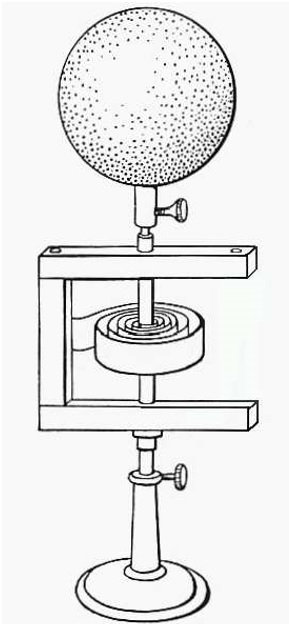
\includegraphics[width=5 cm , height= 10 cm]{Bild2.jpg}
   \caption{Schematische Darstellung des Versuchsaufbau}
\end{figure}
Auf die Achse können verschiedene Objekte angebracht werden.
%Das Eigenträgheitsmoment $I_\text{D}$ sowie die Winkelrichtgröße D lässt sich über die Schwingungsdauer T
%berechnet.
